\documentclass{beamer}
%\usepackage[utf8]{inputenc}
%\usepackage[T1]{fontenc}
%\usepackage[italian]{babel}
\usetheme{Berlin}
\usefonttheme{serif}

\newtheorem{hp}{Ipotesi}
%\newenvironment<>{hp}[1][]{%
	%	\setbeamercolor{Ipotesi}{fg=white,bg=red!75!black}%
	%	\begin{example}#2[#1]}{\end{example}}
\newtheorem{prop}{Proposizione}

\usepackage{amsmath}
\usepackage{mathtools}
\usepackage{url}
\usepackage{hyperref}


%%%%%%%%%%%%%%%%%%%%%%%%%%%%%%%%%%%%%%%%%%%%%%%%%%%%%%%%%%%%%%%%%%%%%%%%%%%%%%%%%%%%%%%%%%%%%%%%%%%%%%%%%%%%%%
%Information to be included in the title page:
\title{Clustering per i gironi \\delle competizioni sportive}
\subtitle{Constrained K-Means Clustering}
\author{Alice Daldossi \\ Massimiliano Ghiotto}
\institute{Università degli Studi di Pavia}
\date

\begin{document}
	
	\frame{\titlepage}
	
\begin{frame}
	\frametitle{Indice}
	\tableofcontents
\end{frame}

\section{K-Means Clustering}
\begin{frame}{K-Means Clustering}
	Siano dati un insieme di $m$ punti $\mathcal{D} = \{\textbf{x}_i\}^m_{i=1}$ in $\mathbb{R}^n$ e un numero $k$ di clusters.
	\begin{block}{Problema del k-means clustering}
		Trovare i centri dei cluster $ \textbf{c}_1, \textbf{c}_2, \dots, \textbf{c}_k  \in \mathbb{R}^n$ tali che la somma della distanza euclidea tra ogni punto $ \textbf{x}_i $
		e il suo centro più vicino $ \textbf{c}_h $ è minimizzato
		\[ \underset{\textbf{c}_1, \dots, \textbf{c}_k}{\min}\, \sum_{i=1}^{m} \underset{h = 1, \dots, k}{\min} \left( \frac{1}{2} \left\| \textbf{x}_i - \textbf{c}_h \right\|^2_2  \right).  \]
	\end{block}
\end{frame}
\begin{frame}
	\begin{block}{Problema del k-means clustering}
		Equivalentemente
		\[ \begin{split}
			\underset{\textbf{c}, T}{\text{min}}&\qquad \sum_{i=1}^{m}\sum_{h=1}^{k} T_{i,h} \left( \frac{1}{2} \left\| \textbf{x}_i - \textbf{c}_h \right\|^2_2  \right) \\
			\text{t.c.}& \qquad\sum_{h=1}^{k} T_{i,h} = 1 \quad i = 1, \dots, m\\
			& \qquad T_{i,h} \ge 0 \quad i = 1, \dots, m,\ h = 1, \dots,k.
		\end{split} \]
	\vspace{-0.5cm}
	Dove 
	\[  T_{i,h} =\begin{cases}
		1 \quad \text{se $ \textbf{x}_i $ è il punto più vicino al centro $ \textbf{c}_h $}\\
		0\quad \text{altrimenti}
	\end{cases} \]
\vspace{-0.4cm}
	\end{block}
\end{frame}
\begin{frame}{Applicazione}
	Un esempio di applicazione di questi metodi è la divisione in gironi delle squadre di serie D che svolgono la Prima Fase Provinciale nella Coppa Italiana del Tennis.	\\
	L'obiettivo è quello di dividere le $n$ squadre in $k$ gironi da $M$ componenti minimizzando la distanza dei circoli di appartenenza.\\
\end{frame}
\begin{frame}
	\begin{columns}
		\begin{column}{0.5\textwidth}
			\begin{center}
				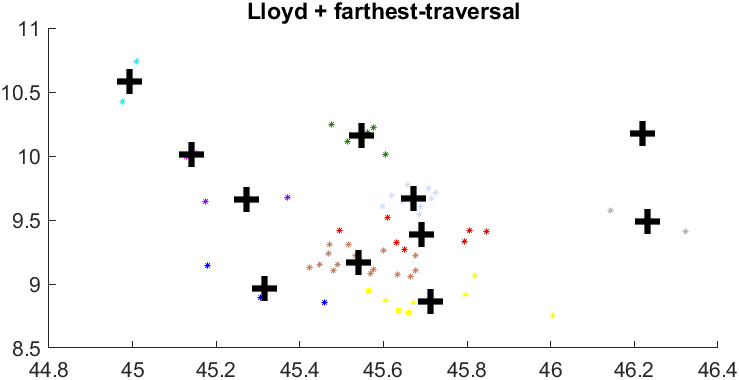
\includegraphics[width=1\textwidth]{lloyd_ft.png}      
			\end{center}
		\end{column}
		\begin{column}{0.5\textwidth}
			\begin{center}
				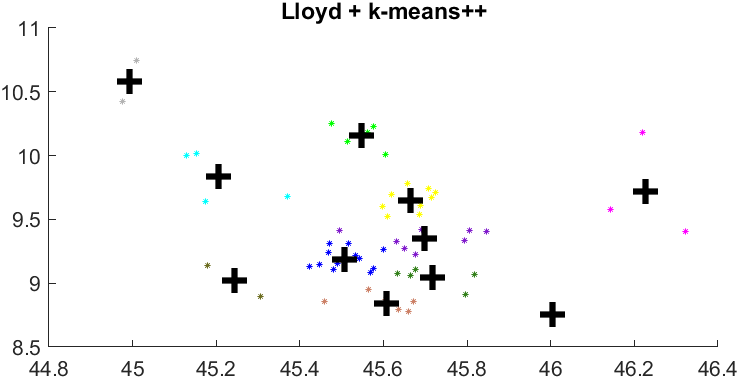
\includegraphics[width=1\textwidth]{lloyd_kmpp.png}      
			\end{center}
		\end{column}
	\end{columns}
	\vspace{0.5cm}
I metodi di k-means clustering trovano soluzioni di minimo locale con cluster vuoti (figura di sx) o troppo scarni. Questo tipo di clustering non va bene per le competizioni sportive, vorremo aggiungere dei vincoli sulla cardinalità dei cluster. \\
I dati raccolti e gli script realizzati sono disponibili al link seguente.
\begin{center}
	\url{https://github.com/MaxGhi8/ProgettoOttimizzazione}
\end{center}
\end{frame}


\section{Constrained K-Means Clustering}
\begin{frame}{Constrained K-Means Clustering}
	Siano dati un dataset $\mathcal{D} = \{\textbf{x}_i\}^m_{i=1}$ in $\mathbb{R}^n$ e un numero $k$ di clusters contenenti almeno $ \tau_h $ punti, dove $ \sum_{h=1}^{k}\tau_h \le m $.
	\begin{block}{Problema del constrained k-means clustering}
		\vspace{-0.8cm}
		\begin{equation}
			\begin{split}
				\underset{\textbf{c}, T}{\text{min}}&\qquad \sum_{i=1}^{m}\sum_{h=1}^{k} T_{i,h} \left( \frac{1}{2} \left\| \textbf{x}_i - \textbf{c}_h \right\|^2_2  \right) \\
				\text{t.c.}&\qquad \sum_{i=1}^{m} T_{i,h} \ge \tau_h \quad h = 1, \dots,k\\
				& \qquad\sum_{h=1}^{k} T_{i,h} = 1 \quad i = 1, \dots, m\\
				& \qquad T_{i,h} \ge 0 \quad i = 1, \dots, m,\ h = 1, \dots,k.
			\end{split}
		\label{CKMP}
		\end{equation}
	\vspace{-0.5cm}
	\end{block}
\end{frame}
\begin{frame}
	\begin{block}{Algoritmo Constrained K-Means Clustering}
			Siano dati un dataset $\mathcal{D} = \{\textbf{x}_i\}^m_{i=1}$ in $\mathbb{R}^n$ e un numero $k$ di clusters contenenti almeno $ \tau_h $ punti, dove $ \sum_{h=1}^{k}\tau_h \le m $; assegnati i centri $ \textbf{c}_{1}^{(t)}, \dots, \textbf{c}_{k}^{(t)} $ della $ t $-esima iterazione, si calcolano i centri $ \textbf{c}_{1}^{(t+1)}, \dots, \textbf{c}_{k}^{(t+1)} $ della $ (t+1) $-iterazione:
			\begin{enumerate}
				\item \textit{Assegnamento cluster:} si trova $ T_{i,h}^{(t)} $ soluzione del problema lineare intero \eqref{CKMP} con centri $ \textbf{c}_{1}^{(t)}, \dots, \textbf{c}_{k}^{(t)} $ fissati;
				\item \textit{Aggiornamento centri:} 
				\vspace{-0.3cm}
				\[ \textbf{c}_{h}^{(t+1)} = \begin{cases}
					\frac{\sum_{i=1}^{m}T_{i,h}^{(t)}\textbf{x}_i}{\sum_{i=1}^{m}T_{i,h}^{(t)}} \quad \text{se} \ \sum_{i=1}^{m}T_{i,h}^{(t)} > 0\\
					\vspace{-0.5cm}\\
					\textbf{c}_{h}^{(t)}\qquad\qquad \text{altrimenti}
				\end{cases} \]
			\end{enumerate}
		\vspace{-0.3cm}
		Si ferma quando $\textbf{c}_{h}^{(t+1)} = \textbf{c}_{h}^{(t)}, \ h=1,\dots,k.$
	\end{block}
\end{frame}
\begin{frame}
	\begin{exampleblock}{Proposizione}
		L'algoritmo Constrained K-Means Clustering termina in un numero finito di iterazioni con un assegnamento dei clusters che è localmente ottimo.
	\end{exampleblock}
	\textit{Dimostrazione.} Siccome esiste un numero finito di modi per assegnare $m$ punti in $k$ clusters tali che, per ogni $h$, il cluster $h$-esimo contiene almeno $\tau_h$ punti, e siccome questo algoritmo non permette assegnazioni ripetute, allora termina in un numero finito di passi.\\
	Inoltre, ad ogni iterazione la funzione obiettivo diminuisce strettamente; in particolare, quando l'algoritmo termina, questa funzione obiettivo \eqref{CKMP} non può essere diminuita né riassegnando i punti a clusters diversi, né definendo un nuovo centro, quindi la soluzione raggiunta è localmente ottima.\vspace{-0.5cm}\begin{flushright}$ \square$\end{flushright}
\end{frame}

\subsection{Sotto-problema dell'assegnamento dei clusters}
\begin{frame}{Sotto-problema dell'assegnamento dei clusters}
	\begin{columns}
		\begin{column}{0.5\textwidth}
			Lo step \textit{assegnamento cluster} può essere scritto in modo equivalente come un problema di ottimizzazione lineare intera per la ricerca del flusso di costo minimo (MCF).  
		\end{column}
		\begin{column}{0.5\textwidth}
			\begin{center}
				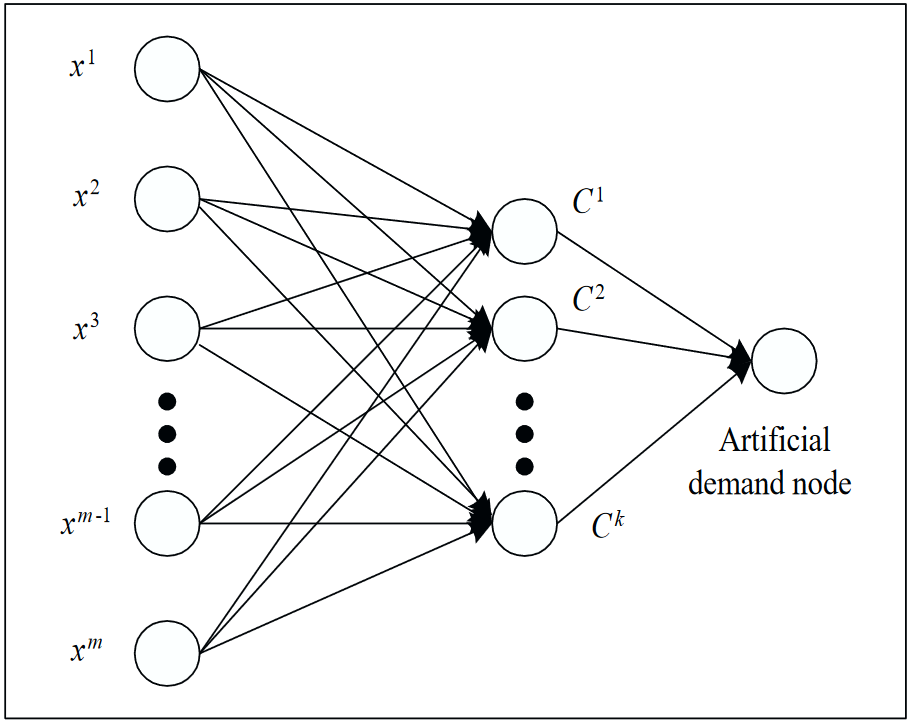
\includegraphics[width=1\textwidth]{MCF.png}      
			\end{center}
		\end{column}
	\end{columns}
	\vspace{0.3cm}
	Siano $\mathcal{N} = \{\textbf{x}_i\}_{i=1}^m \cup \{\textbf{c}_h\}_{h=1}^k \cup \{a\}$ l'insieme dei nodi e $\mathcal{A} = \{(\textbf{x}_i,\textbf{c}_h), \ \textbf{x}_i,\textbf{c}_h \in \mathcal{N}\} \cup \{(\textbf{c}_h, a), \ \textbf{c}_h \in \mathcal{N}\}$ l'insieme degli archi orientati. 	
\end{frame}
\begin{frame}
	Ad ogni \textit{nodo-fornitore} $\textbf{x}_i$ è associato un valore $b_{\textbf{x}_i}=1$, ad ogni \textit{nodo-richiesta} $\textbf{c}_h$ un valore $b_{\textbf{c}_h}=-\tau_h$ e al nodo artificiale $a$ un valore $b_a = -m+\sum_{h=1}^k \tau_h$. \\
	Il costo dell'arco $(\textbf{x}_i, \textbf{c}_h)$ è $c_{i,h} = \left\| \textbf{x}_i - \textbf{c}_h \right\|^2_2 $, mentre quello degli archi del tipo $(\textbf{c}_h, a)$ è nullo.
	\begin{block}{MCF}
		Siano $y_{i,j}$ le variabili che indicano l'ammontare di flusso sull'arco $(i,j) \in \mathcal{A}$. Il problema $MCF$ è il seguente:
		\begin{equation} \label{MCF}
			\begin{split}
				\underset{y}{\text{min}} & \qquad \sum_{(i,j)\in\mathcal{A}} \textbf{c}_{i,h}y_{i,j}\\
				\text{t.c.} & \qquad \sum_{j} y_{i,j} - \sum_{j} y_{j,i} = b_i, \ \forall i \in \mathcal{N}\\
				& \qquad 0 \le y_{i,j} \le m, \ \forall (i,j) \in \mathcal{A}
			\end{split}
		\end{equation}
	\vspace{-0.5cm}
	\end{block}
\end{frame}
\begin{frame}
	\begin{exampleblock}{Proposizione}
		Se per ogni $h=1,\dots,k$, $\tau_h$ è un intero, allora esiste una soluzione ottima del problema \eqref{MCF} tale che $T_{i,h} \in \{0,1\}$.
	\end{exampleblock}
	\textit{Dimostrazione.} 
	Siccome si tratta di un problema di ottimizzazione lineare intera per la ricerca del flusso di costo minimo con tutti i pesi associati ai nodi interi allora, per i risultati di programmazione lineare intera, esiste sempre una soluzione ottima e intera. \\
	Dato che per l'assegnazione dei cluster i valori di $ T_{i,h} $ corrispondono a $ y_{\textbf{x}_i, \textbf{c}_h} $ e ogni nodo $ \textbf{x}_i $ ha disponibilità pari ad $ 1 $, allora $ T_{i,h} \in \{0,1\} $.\vspace{-0.5cm}\begin{flushright}$ \square $\end{flushright}
\end{frame}

\section{Conclusione}
\begin{frame}{Conclusione}
	\begin{exampleblock}{Osservazione}
		Dal metodo del constrained k-means clustering si può ottenere il metodo del k-means prendendo $\tau_h=0, \ \forall h=1,\dots,k$.
	\end{exampleblock}
	\begin{exampleblock}{Osservazione}
		In generale, aggiungendo vincoli ad un problema di minimizzazione si restringe la regione ammissibile, dunque il valore della soluzione ottima globale aumenta.\\
		Inaspettatamente, l'approccio constrained k-means clustering, nonostante richieda vincoli aggiuntivi rispetto a quello del k-means clustering, è meno propenso a convergere a minimi locali, fornendo una migliore rappresentazione dei dati.
	\end{exampleblock}
\end{frame}
\begin{frame}{Applicazione}
	I dati raccolti e gli script realizzati sono disponibili al link seguente.
	\begin{center}
		\url{https://github.com/MaxGhi8/ProgettoOttimizzazione}
	\end{center}
	 
\end{frame}

\end{document}